% template-v1.tex: LaTeX2e template for Usenix papers.
% Version: usetex-v1, 31-Oct-2002
% Revision history at end.

%\documentclass[preprint,natbib,tenpoint,times]{sigplanconf}
\documentclass[final]{usetex-v1}

% These packages are optional, but useful
\usepackage{epsfig}     % postscript figures
\usepackage{url}        % \url{} command with good linebreaks
\usepackage{multirow}
%\usepackage{subfig}
\usepackage[usenames,dvipdfm]{color}

\begin{document}

\title{Evolving Directory Model, Storage Structures, and Interface for Large Scale Small File Access}

%"Everything should be made as simple as possible, but no simpler." -Einstein

% authors.  separate groupings with \and.
%\authorinfo{Can Ma$\,^{1,2}$, Jin Xiong$\,^{1}$, Dan Meng$\,^{1}$}{
%$\,^{1}$National Research Center for Intelligent Computing Systems,\\
%Institute of Computing Technology, CAS, Beijing, China, 100190\\
%$\,^{2}$Graduated School of Chinese Academy of Sciences, China, 100049
%}{\{macan,xj,md\}@ncic.ac.cn}

\author{
%\authname{Can Ma$\,^{1,2}$, Jin Xiong$\,^{1}$, Dan Meng$\,^{1}$, Weiping Wang$\,^{1}$}
\authname{Can Ma, Jin Xiong, Dan Meng, Weiping Wang, Jizhong Han}
\authurl{\url{{macan,xj,md,wpwang}@ncic.ac.cn}}
%\authaddr{$\,^{1}$National Research Center for Intelligent Computing Systems,}
\authaddr{National Research Center for Intelligent Computing Systems,}
\authaddr{Institute of Computing Technology, CAS, Beijing, China, 100190}
%\authaddr{$\,^{2}$Tencent Inc. , Shenzhen, China}
} % end author

%\author{\textit{Author Names Removed for Reviewing}\\
%{\texttt{Draft}}}

\maketitle

\begin{abstract}
    In emerging popular Web applications, e.g. online photo galleries, documents and social network services, large scale small files are concurrently created and read. These applications exhibit low latency requirements for accessing massive small files. Particularly, \emph{N-Form} and \emph{1-N Mapping} issues of distributed file systems, that affect I/O performance of small files, have not been addressed yet.

    In this paper, we propose to use tabular directory model, structured storage and tabular query interface to address \emph{N-Form} and \emph{1-N Mapping} issues to boost up small file handling. We implement a prototype file system to manage billions of small files, and focus on improving metadata scalability elastically and exploiting locality and parallelism to improve small file I/O.

    Our evaluation demonstrates that the new directory model, storage structures, and interface can not only save storage space, but also increase small file I/O performance. With 32 servers, we deliver the leading metadata and small file I/O performance: 180,000 file creates per seconds and 1GB/s write bandwidth.
\end{abstract}

%\keywords{Small Files, N-Form, 1-N Mapping, Extendible Hashing, Semantic Data}

\section{Introduction}

    % Motivation: Problem 1: N-Form; Problem 2: 1-n Mapping( Out of core indexing)
    Emerging Web applications, e.g. online photo, audio, video, document and social network services, exhibit very different data access and storage requirements from HPC applications. Lots of small files are created, processed, and returned every second. For example, Facebook, maintained over 260 billions of photos and provided a peak access throughput of 550K photos per second in 2010\cite{facebook-haystack}. Taobao, a famous e-commercial site in China, maintained over 20 billions of photos with average photo size at 15KB\cite{taobao-tfs}. Renren, a popular social network in China, maintained billions of files with average file size at 32KB\cite{trf}. And geographic information services (GIS), e.g.  Google Maps and OpenStreetMap, rely on billions of map tiles(a few KB to hundreds KB) to serve. With the evolution of Web 2.0, application requirements of storing and accessing billions of small files are increasing. The typical characteristics of small file access are: \textbf{a)} lots of small files, \textbf{b)} concurrent file creations and reads, and \textbf{c)} little file modifications. We can foresee that Web applications in the next few years require scalable distributed storage systems that can efficiently write, read and process on billions or even trillions of small files, and provide low latency query (or search) interface to them. However, as far as we know, most file systems can not handle small files as efficient as handle large files. Classic distributed file systems are designed to optimize I/O bandwidth for large files rather than to optimize latency for small files. Besides this, Web applications had exposed another two problems which make things even worse.

    \textbf{Problem A}: (\textit{N-Form}) Many Web applications need to store \textit{N} forms of the original file. For example, online photo galleries need to store several different resolutions of an image for previews. HayStack, developed by Facebook to store user photos, keeps the original image and three different sized thumbnails\cite{facebook-haystack}. Video services, e.g. Youtube, need to store many key frames of a video to serve user previews. Online document sites, e.g. Google Doc, need to keep summary page and preview pages for each document. For these files that derived from one file, saving them in independent files means that \emph{N} copies of \emph{almost-the-same} metadata are generated. It not only wastes space, but also tenses the metadata service. And data access performance is also penalized by random seeking among these files.

    \textbf{Problem B}: (\textit{1-N Mapping}) Most distributed file systems map a file in its namespace to \emph{one} or \emph{N} files in local file systems. For example, in Lustre\cite{lustre}, PVFS2\cite{pvfs} and Ceph\cite{ceph}, file data is stored into one (for small file) or several files (for large file) of storage node's local file system. It means that each file data access requires at least one metadata lookup in local file system. Although this out of core indexing has little impact on large file access, it greatly increases the I/O latency for small files.

    In this paper, we evolve the classic directory model, storage structures, and interface to address the above small file access issues. We propose a tabular directory model and query interface for \emph{N-Form} problem, and directory based file aggregation and structured store for \emph{1-N Mapping} problem. The tabular directory model groups \emph{N} forms of a file together to reduce metadata footprint and mitigate service stress. And, directory based aggregation eliminates out of core indexing to reduce I/O latency. We focus on improving metadata scalability elastically, and exploiting locality and parallelism to accelerate small file I/O. We evaluate these methods in a prototype file system, \textit{PomegranateFS}(abbr. PFS), to reveal the practical effects.

    % Contribution
    Our main contribution is that we evolve a new tabular directory model, storage structures, and query interface for large scale small file access. It solves \textit{N-Form} and \textit{1-N Mapping} problems for typical Web applications and gets best-in-class small file performance.

    In the rest of the paper, we presents the motivations and related works in Section 2, design issues in Section 3, implementation details in Section 4, evaluation results in Section 5, and conclusion in Section 6.

\section{Motivation and Background}

    Over the last two decades, research in distributed file system was mainly driven by application workloads that emphasized on large files. Few researches optimized small file access performance in specific file systems\cite{cffs,reiserfs,giga,ipdps09,europar08}. And most file system cannot handle large scale small files efficiently. This section summaries the technology trends calling for large scale small file access and how current file systems are ill-suited to satisfy this call.

\subsection{Motivation}

    % Give a photo gallery's example and talk about other design alternatives.
    In today's social networks, photo gallery is an important I/O workload. For instance, massive users of QZone \footnote{A large social network based on the popular instant messaging network (QQ), which has more than 100 millions active users.} upload tens of millions photos every day. For each photo, at least \emph{three} different sized (small, medium, and original) images have to be saved. Typically, file sizes are under 1 MBs, from a few KBs to hundreds KBs. These different sized photos has special purposes. The small one is used as a thumbnail for gallery previews. The medium one is used in list previews. And the original one is used for downloading. Web site keeps gallery metadata and photo lists in relational database but image files in distributed file system (DFS), because saving these images in database is both inconvenient for management and inefficient for access. Generally, storing these images in current distributed file system means that for each uploaded photo we have kept \emph{three} files' metadata in DFS's namespace and another \emph{three} in underground local file systems. The first amplification is the \emph{N-Form} issue: redundant metadata of DFS. Keeping redundant metadata means that DFS has to use more storage space to save, more I/O bandwidth to load, more memory to cache, and more requests to serve. The second amplification is the \emph{1-N Mapping} issue: redundant metadata of local file system. For each DFS file read, user has to firstly look for metadata in the local file system, and secondly read in the data content. It harms the I/O latency of small files.

    Photo galleries, although important, might not be a sufficient reason for overhauling current file system implementations. Yet there are diverse applications, such as multimedia storages, online document workspaces, GIS applications and gene sequencing, that want to save large scale small files. Although these applications are often using the file system as a lightweight ``key/value store'', replacing file systems with NoSQL databases\cite{cassandra,hbase} is an oft-rejected option because it is undesirable to port existing code to use new API (e.g. KV) and because many NoSQL databases do not provide sufficient small data read or write latency\cite{ycsb}.

    To boost up small file access in distributed file systems, we have to remove metadata redundance and eliminate unnecessary file mappings. Unfortunately, current file system directory model (key/value) is not capable to pack files with one file name easily, and the storage structure does not do aggregations aggressively. Although there are many researches on small file access, few research has focus on \emph{N-Form} and \emph{1-N Mapping} issues that introduced by emerging Web applications.

\subsection{Related Works}

    Large scale small file access is non trivial, especially for file systems that want to support both small file and large file efficiently. For large file access, data content transfer latency dominates the total latency. While, for small file access, data content is short, and the transfer latency is tiny. The latency of metadata access and disk rotation for data have a huge impact on total latency.

    File systems, which split metadata as \texttt{dentry} and \texttt{inode}, performs bad on small files. Each file access has to lookup at lease three disjointed positions, \texttt{dentry}, \texttt{inode}, and \texttt{block}, to get the data. As a result, numerous random accesses are generated with concurrent file access. And these random accesses further increase the rotation latency. Thus, C-FFS\cite{cffs} and Ceph\cite{ceph} embedded file \texttt{inode} in \texttt{dentry} to eliminate indirect access in file lookup stage. ReiserFS\cite{reiserfs} tailed small file data with metadata to eliminate indirect access in data read stage. Although combining \texttt{dentry} and \texttt{inode} has complicated hard link implementation, it has improved small file performance a lot. We evolve this idea further to combine some file metadata, small file content, and attributes together to decrease latency.

    Lots of small files also overwhelm directory indexing structures. Classic B+ tree is used in Ext3, Lustre and many other file systems. It is $O(log_{k}N)$ and terrible slow for large directories. Thus, GIGA+\cite{giga} and SkyFS\cite{skyfs} had proposed to use extendible hashing\cite{eh} to manage large directories. These works are valuable for us to build a low latency $O(1)$ metadata service.

    On the other hand, small file access means lots of random I/Os. When creating small files, blocks are allocated before doing I/O operations. And when doing I/Os, writes are somewhat randomized. It is fairly slow for hard disks. Thus, file systems, e.g. hFS\cite{hfs}, use log structured file format to aggregate small files and flush them as a whole to reduce disk rotations and utilize sequential I/O bandwidth. We carry on this idea and design a scatter and aggregation approach to set up many sequential data flows to make use of locality and parallelism.

    For distributed file systems (abbr. DFS), things are even worse. DFS need another access stage on storage nodes' local file systems. For example, in Lustre\cite{lustre}, PVFS\cite{pvfs}, and Ceph, file content is distributed on a set of nodes with a specific local file name. For each read, storage server has to lookup, open, read, and close the local file. It is inefficient for latency sensitive small file read. Thus, Michael et al.\cite{europar08} had proposed to remove the metafile in PVFS, which is not needed for small file, to improve small file performance. Philip et al.\cite{ipdps09} had integrated five approaches, e.g. batched metadata commit and new I/O flows, together to improve small file performance. However, these researches hasn't essentially solved the problem of file mappings between DFS and local file system. While, we propose a new directory based file aggregation approach to remove unnecessary mappings.

    Researchers\cite{hotcloud,gfs} had proposed to use table interface to solve small files' problems. However, these works were fragmented and had not integrated and evaluated in one system. Besides, comparing with columnar databases\cite{cstore,cassandra,hbase}, we have a similar column oriented table model. However, our directory table is schema-less and can be altered dynamically, and the storage structures are optimized for unstructured data access.

    In all, although researches had addressed some issues of small files, they hadn't solved the \textit{N-Form} and \textit{1-N Mapping} problems fundamentally. Combining metadata and data or using log structured file format, has no effect on eliminating redundant metadata, and didn't solve the \textit{N-Form} problem. Similarly, approaches proposed for PVFS have not eliminated file mappings, and didn't solve the \textit{1-N Mapping} problem.

\section{Design Issues}

    To address \emph{N-Form} and \emph{1-N Mapping} issues and build an efficient small file store, we focus on evolving directory model, storage structures, and interface. To minimize space consumption of DFS metadata, we propose a tabular directory model to group similar files together. To store small files efficiently, we propose a directory based storage structure to scatter and aggregate files based on columns. Finally, to access these columns of files more easily and quickly, we propose a new query interface and support searching.

\subsection{Tabular Directory Model}

    % current directory model vs evolved directory model
    Generally, directory of current file system is a plain (key/value) table with three columns: \emph{name}, \emph{metadata} (including extended attributes, abbr. xattr), and \emph{data}. Typically, for several sized images from one photo, each image is saved in a standalone file, shown by Figure \ref{directory_model}(a). Then, we have \emph{N} copies of file metadata. Alternatively, we can use xattr to pack these \emph{N} images together to eliminate redundant metadata and boost up metadata accessing. However, it is non-trivial to store several files with one name in plain directory model. Firstly, it's impossible to store large data content in xattr. Linux VFS \texttt{xattr} only supports setting and getting at most 64KB buffer. Even worse, local file system, e.g. Ext3, sets up a smaller buffer limit at 4KB. Secondly, user has to pack multiple image files into data content and record offset and length of each image in xattr, shown in Figure \ref{directory_model}(b). Although this approach is possible to save \emph{N} image files under one name, it is inconvenient for users. Other applications have to build their own packing and unpacking framework.

\begin{figure}
  % Requires \usepackage{graphicx}
  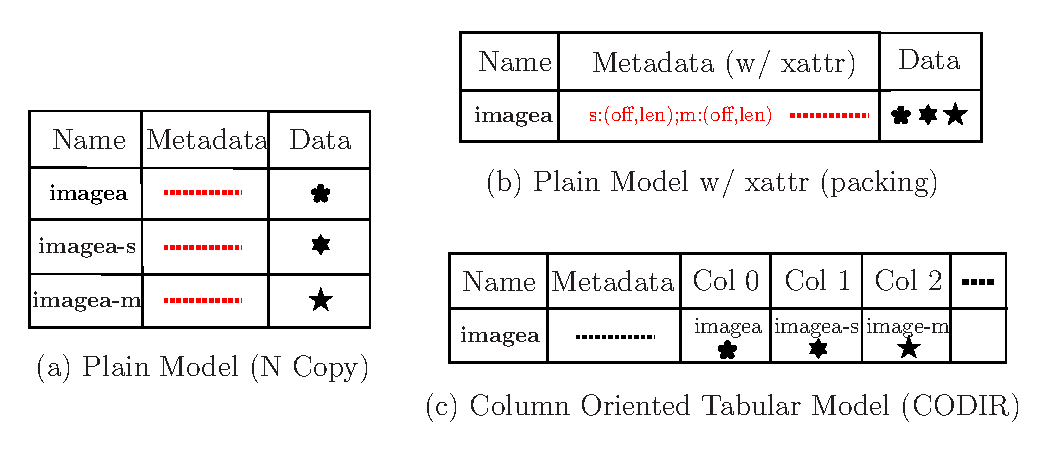
\includegraphics[width=.5\textwidth]{directory_model.eps}
  \caption{Directory Model for N-Form Problem. \textit{\small Imagea-s and imagea-m are the small and medium forms of imagea. Plain directory model is either (a) metadata costing or (b) difficult to use. Column oriented tabular model resolves both these difficulties.}}\label{directory_model}
\end{figure}

    To address the \textit{N-Form} issue, we propose a column-oriented tabular directory model (abbr. CODIR). Shown by Figure \ref{directory_model}(c), each file has two basic columns: \emph{name}, and \emph{metadata}; and multiple \emph{data columns}: different file forms, xattrs, or tags. Thus, several file forms derived from one file can be stored in different columns under one file name. For example, all file forms origin from \textit{imagea} are saved with name \textit{imagea}. Each form (e.g. \textit{imagea-s}, the small sized \emph{imagea}) is saved in one column (e.g. \textit{Col 1}). By utilizing this tabular directory model, users can not only save space, but also store and retrieve column data much more easier. We have proposed an API to access file columns in Section \ref{interface}.

    \subsubsection{Handle Sparse Table}

    In CODIR's table, there might be many columns. If columns' metadata are saved in dentries, then dentries are variably sized. Directory operations such as \texttt{seekdir} would be difficult to implement. Thus, we make dentry has a fixed size. Each dentry contains fixed number of \emph{direct} columns and many \emph{indirect} columns. Frequently accessed data should be put in direct columns, while infrequently accessed ones should be put in indirect columns.

    Since directory contains lots of columns, it might be sparse. Some dentries do not have valid values for some columns. Obviously, these blank cells do not need to be saved. For each column, valid data are sent to storage server and aggregated in column files, shown by Figure \ref{storage_engine_model}. And data written offsets must be kept in dentries (as metadata) for future read and write. Data offsets of direct columns are stored in dentries, while data offsets of indirect columns are stored in an \emph{indirect file}. Thus, accessing data of direct columns are faster than that of indirect columns. Besides, if the table is sparse, it is space consumptive for indirect columns to keep these offsets in a fixed sized array with holes. Thus, the indirect file is append-only with a tail index record. For each update, the updated offset and an index record (indicates column ranges and internal offsets) are appending to tail of the file. On reading, the index record is read in firstly to determine which file position should be read next.

    Although CODIR supports sparse table, we argue that sparse tables decrease directory performance and waste more space. To reduces sparse tables in practice, users should only group files with similar properties in one directory. For example, store user photos and documents in separated directories. Fortunately, this simple rule always keeps because we classify things before storing.

    %Each directory has a schema to describe what has been stored in each column. The schema can be altered dynamically, while the column data stays the same.

    \subsubsection{Advantages of CODIR}

    CODIR deduplicates DFS's metadata for \emph{N-Form} problem. Other than metadata saving, it has some other advantages. Firstly, it is more efficient to store large data than xattr. In many file systems, \texttt{xattr} attaches to file metadata, and is not effective at storing large data. While, CODIR permits to store several variable length of data in it. And these data are not required to store with metadata. Secondly, it is more efficient to do data compression on columns. Shown by Figure \ref{storage_engine_model}, we aggregate one or several columns' content (e.g. \emph{Metadata}) to one storage file. Thus, in each directory, we have already grouped similar data together. It is efficient for compressor to get a better zip ratio. For example, we had compressed the \emph{Metadata} file for about \emph{25 times} smaller by using LZO\cite{lzo} in PFS. Thirdly, it is more efficient to do bulk load on specific columns. For example, file content of the same column are stored in the same storage file, thus, it is suit for bulk loading. This is valuable for Web applications that needs bulk file loads in the cache filling stage. For example, in photo galleries, loading small sized images (aka thumbnails) to cache are very fast with CODIR, because these are all sequential I/Os.

\subsection{Structured Storage}

\begin{figure}
  % Requires \usepackage{graphicx}
  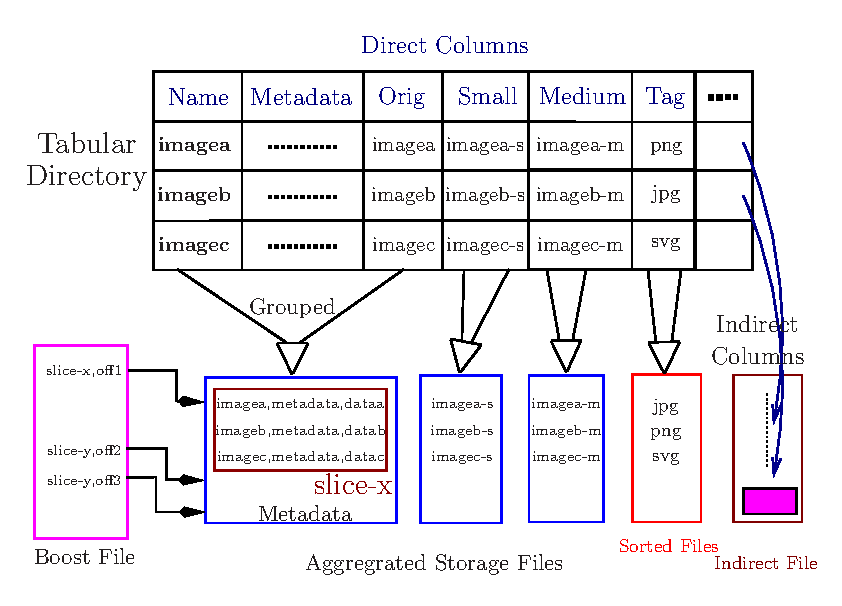
\includegraphics[width=.5\textwidth]{storage_engine_model.eps}
  \caption{Storage File Mappings. \textit{\small The first three columns are grouped and aggregated as one storage file, the next two columns are aggregated as independent storage files, and the Tag column is saved in a sorted file. Boost File accelerates metadata access. Indirect file contains indirect columns' metadata.}}\label{storage_engine_model}
\end{figure}

    % eliminate 1-N mapping: directory-based data aggregation; column-oriented model directed columnar store;
    Current distributed file systems mostly map their files to files of local file system on storage nodes. Thus, even you resolve the \emph{N-Form} problem, you still have the \emph{1-N Mapping} problem that increases small file access latency. Shown by Figure \ref{storage_engine_model}, to reduce storage file metadata lookup latency, we propose a directory-based file aggregation approach. This aggregation reduces metadata of local file system, and is not only saving disk space but also saving memory (no need to cache lots of dentires of local file system). Small files in one directory are logically grouped in a big storage file to eliminate redundant metadata. Each data access is actually a read or write in this big file. Thus, ideally, for each directory, we only have to lookup and open one storage file. By caching this file's metadata, data I/O of small files does not need to do metadata lookups in local file system thereafter. Meanwhile, a file system directory is naturally a locality set. Files in one directory might be accessed contiguously. Aggregating files of the same directory not only doesn't ruin, but also improve the spatial locality.

    At the same time, in CODIR, data contents are aggregated by column by default. The rationale of splitting file columns into several storage files is to reduce unnecessary data loading in column fetching (and prefetching). For example, in a photo gallery, when you visit a photo list (previews), it is unnecessary and time consuming to read in every photo's original file. However, co-accessed columns could be grouped and stored together. For example, in Figure \ref{storage_engine_model}, we group file's metadata and original data together. Each file lookup, that read-in the metadata, would prefetch the data content to cache either. Subsequent data access would hit in the cache.

    \subsubsection{Aggregated Storage Files}

    We use log structure storage format for the aggregated file data. For small files, it is more space efficient than block based storage format because of no internal fragments\cite{lfs}. New arriving data is appended to tail of the file. Removing files are only metadata operations and do not need to update the data file. Every small file write must contain the full file content. Thus, file rewrite has to be transformed to read-modify-write (RMW).

    After lots of file deletions or modifications, the aggregated data file might be filled with holes. To save storage space, these holes have to be detected and garbage collected (GC). For each directory, metadata that needed in GC has already co-located with the data. Thus, the GC process could run incrementally against directories on each storage node to not interfere with storage process.

    The RMW issue of file rewritten might be a performance bottleneck. However, in Web applications, there are fewer file rewritten than file creations and reads. Further more, \texttt{a)} read small file (in stage R) means less time to stall, and \texttt{b)} lots of rewritten are actually issued after file reads (which matches the order of stages R and M). Thus, we argue that RMW issue has more impacts on larger files than smaller ones and it is worth sacrificing rewrite performance to optimize file creation and read.

    \subsubsection{Structured Storage Files}

    Dentries are stored in an aggregated storage file: \emph{Metadata}. Number of dentries are grouped as a \emph{slice}, which is the basic metadata read and write unit. Slice is different from directory partition in GIGA+\cite{giga} and SkyFS\cite{skyfs}. Directory partition uses out-of-core indexing, while slice use hash table indexing. It reduces access latency for small files by eliminating out-of-core indexing.

    It is slow to do slice lookups in the log structure \emph{Metadata} file. Thus, an index file is built, \emph{Boost File}, for the metadata file to speed up lookups. The index keeps a record $<$slice, offset$>$ for each active slice. \emph{Boost File} is a supplement of \emph{Metadata} file. It is guaranteed to be updated on every slice write. Even if corrupted, it can be regenerated by scanning \emph{Metadata} file. Slice in \emph{Metadata} file has a header, which contains magic numbers and special inequations (e.g. length restraint). These can be used as border markers of slice in scaning.

\begin{figure}
  % Requires \usepackage{graphicx}
  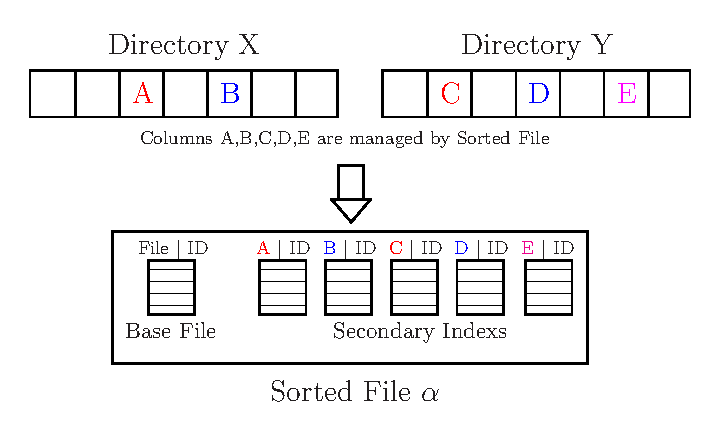
\includegraphics[width=.5\textwidth]{index_mapping.eps}
  \caption{Sorted File Format. \textit{\small Some columns of directory X and Y are directed to Sorted File $\alpha$. Each Sorted File contains one base file and several secondary indexes.}}\label{index_mapping}
\end{figure}

    Semantic searches, e.g. ``\textit{Top-K query: find the K hot jpeg files}'', are widely used in many applications\cite{spyglass,smartstore}. In CODIR, columns could be used to store application specific tags or xattrs. These tags and xattrs are used to serve semantic searches. Researches\cite{spyglass,smartstore} have found that using an external database ruins the spatial query locality, and proposed many semantic search approaches on large scale file systems. However, most of these approaches depend on offline file scanning, and are not capable to handle heavy mutable file systems (for Web2.0 applications). To support online indexing, we propose to \textbf{1)} use internal \emph{sorted} file instead of external database, \textbf{2)} use Star schema to maintain relationships among columns, and \textbf{3)} only manage user-defined subset of directory columns to decrease file subset size that we handle. At the same time, sorted file is tightly coupled with file system to achieve lower latency. For example, shown by Figure \ref{index_mapping}, columns \emph{A, B} from directory \emph{X}, and columns \emph{C, D, E} from directory \emph{Y} are kept in one sorted file \emph{$\alpha$}. Each sorted file contains a base file to save basic mappings from file name to unique file id (File$|$ID), and several secondary indexes for each column (e.g. A$|$ID). In this way, it is elastic to add new columns or delete old columns. Sorted files could be implemented by key/value stores such as BerkeleyDB\cite{berkeleydb}. In all, sorted file not only maintains spatial locality, but also provides more flexibility. Thus, in Figure \ref{storage_engine_model}, query ``\textit{find all the jpeg files}'' can be executed by searching the \emph{sorted} file and locating file \emph{imageb} directly, rather than scanning the whole directory to find the file.

\subsection{Tabular Query Interface}
\label{interface}

    % exploit the existing xattr interface: getxattr, setxattr, listxattr, ...
    Firstly, as we have extended the directory model to store multiple columns, we need an interface to manipulate table cells. Secondly, in large file systems, searching is more efficient than directory traversing to find a file subset. As a result, we provide a user level table manipulation interface, and wrap it to fit the \texttt{xattr} interface: \texttt{getxattr} and \texttt{setxattr}.

    \begin{table}[t]
    \centering
    \begin{tabular}{c|l}
      \hline
      Category & Prototype\\
      \hline
      \hline
      table & \texttt{\scriptsize tab\_t \textbf{opentab}(char *dir)}\\
      & \texttt{\scriptsize \textbf{closetab}(tab\_t th)}\\
      & \texttt{\scriptsize \textbf{tabschema}(tab\_t th, colid, colname)}\\
      & \texttt{\scriptsize \textbf{readtab}(tab\_t th, file,\emph{\color{red}colname},buf,len)}\\
      & \texttt{\scriptsize \textbf{writetab}(tab\_t th,file,\emph{\color{red}colname},buf,len)}\\
      & \texttt{\scriptsize \textbf{bulkload}(tab\_t th, \emph{\color{red}colname}, buf, len)}\\
      \hline
      raw & \texttt{\scriptsize \textbf{tread}(filepath, \emph{\color{red}colid}, off, buf, len)}\\
      & \texttt{\scriptsize \textbf{twrite}(filepath, \emph{\color{red}colid}, off, buf, len)} \\
      \hline
      sorted & \texttt{\scriptsize sorted\_t \textbf{opensorted}(char *name)}\\
      & \texttt{\scriptsize \textbf{closesorted}(sorted\_t s)}\\
      & \texttt{\scriptsize \textbf{search}(sorted\_t s, char *expr) //+{\color{red}\textbf{JOIN}}}\\
      & \texttt{\scriptsize \textbf{set}(sorted\_t s, filepath, char *kvlist)}\\
      & \texttt{\scriptsize \textbf{delete}(sorted\_t s, filepath, char *key)}\\
      & \texttt{\scriptsize \textbf{update}(sorted\_t s, filepath, char *kv)}\\
      & \texttt{\scriptsize \textbf{test}(sorted\_t s, filepath, char *key)}\\
      \hline
      \hline
      getxattr & Wrapper Examples\\
      & \texttt{\scriptsize (filepath, \textbf{EMBEDDED\_CMD\_STRING}, buf,len)}\\
      \hline
      \texttt{\scriptsize opentab} & \texttt{\scriptsize "pfs.table.opentab.DIR"}\\
      \texttt{\scriptsize bulkload} & \texttt{\scriptsize "pfs.table.bulkload.TH.colname"}\\
      \texttt{\scriptsize search} & \texttt{\scriptsize "pfs.sorted.search.S.R:$k1<10\&k2>20$"}\\
      \hline
      \hline
      setxattr & Wrapper Examples\\
      & \texttt{\scriptsize (filepath, \textbf{EMBEDDED\_CMD\_STRING}, buf,len)}\\
      \hline
      \texttt{\scriptsize writetab} & \texttt{\scriptsize "pfs.table.writetab.TH.file.colname"}\\
      \texttt{\scriptsize set} & \texttt{\scriptsize "pfs.sorted.set.S.file.k1=v1,k2=v2"}\\
      \hline
    \end{tabular}
    \caption{User Level Interface and xattr Wrapper}
    \label{tabular_interface_table}
    \end{table}

    As shown by Table \ref{tabular_interface_table}, we defined three API groups for CODIR. The \textbf{table} group is for applications. When opening the directory table, user can read, write and do bulk load on specific column. The \textbf{raw} group is for library developers. They can read/write specific file column by column ID directly instead of name. The \textbf{sorted} group is for tag operations. A list of key/value pairs can be attached with each file. KV pairs from specific columns of directories are grouped in one sorted file. These pairs are automatically indexed. Thus, by utilizing sorted files, queries and joins on file tags are more fast than brute-force scanning the whole directory tree.

    The \texttt{xattr} wrappers encode tabular operations in strings. For example, string ``pfs.sorted.set.S.file.k1=v1, k2=v2'' represents adding tuple $<$file, k1=v1;k2=v2$>$ to sorted file \texttt{S}. String ``pfs.sorted.search.S.R: $k1<10\&k2>20$'' represents a range (\texttt{R:}) search on sorted file \texttt{S} that satisfies $k1<10\&k2>20$. Search results are returned as \emph{iterator} to allow users to iterate on.

\section{Implementation Details}

\begin{figure}[t]
  % Requires \usepackage{graphicx}
  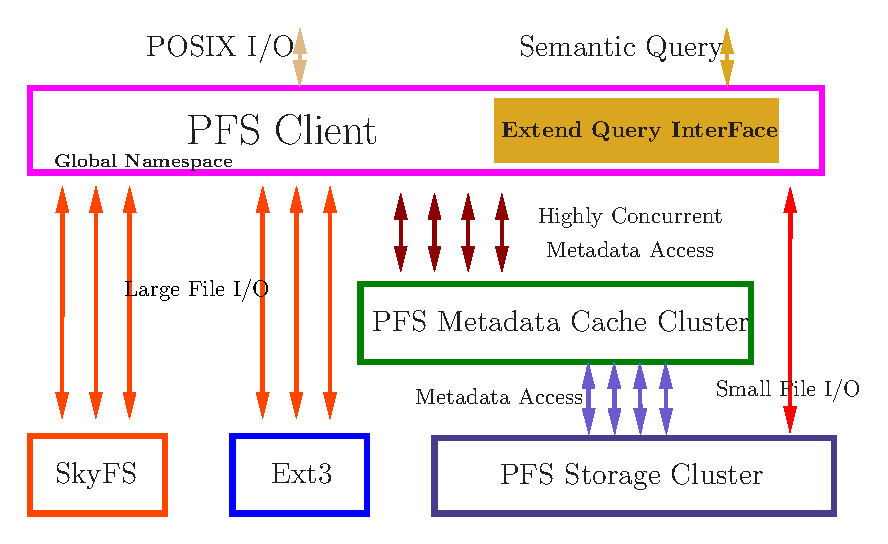
\includegraphics[width=.5\textwidth]{hvfs_architecture3.eps}\\
  \caption{Architecture of PFS}\label{hvfs_architecture}
\end{figure}

    We have implemented CODIR, structured storage, and tabular interface in a prototype distributed file system PFS for Web applications that need to access large scale small files. Large files are handled by other DFSs. Shown by Figure \ref{hvfs_architecture}, PFS contains a FUSE\cite{fuse} client, a dedicated metadata and storage cluster to handle small files, and Ext3, SkyFS (or Ceph, PVFS2) store to handle large files. However, CODIR could be implemented in other DFSs to improve their small file performance.

    The metadata cluster is a collaborative cache layer over storage servers to provide low latency metadata service. Metadata modifications are flushed back to disk asynchronously. The metadata service latency dominates the whole file access latency for extremely small files. As a result, caching metadata in memory decreases the total latency greatly.

    The storage cluster is a shared storage pool. Metadata and data of small files are scattered to all the servers and aggregated by directory. Thus, for each directory, sequential data write flows are set up on every server to exhaust large scale concurrent file creations.

\subsection{Distinguish Small Files}
    % static or dynamic
    Typically, small files are less than 1MB\cite{gfs}. In many photo galleries, we found that the average file size is 32KB\cite{trf}. Thus, we make 2MB as the transition point from small file to large file for higher degree of confidence. At file \texttt{open} time, there is no hint on file length. There are two approaches to distinguish small files. The first one is a \emph{static} approach. Parent directory is marked as \emph{static-small} and all file creations in it automatically inherit the property. The second one is a \emph{dynamic} approach. Parent directory is marked as \emph{dynamic-small}. Static-small doesn't allow automatic transformation from small file to large file, while dynamic-small allows that.

    At \texttt{open} time, we use parent directory's property to guide subsequent I/O operations. When it is static-small, the followings are all small file operations. When it is none, the following are all large file operations. When it is dynamic-small, PFS client probes on each file write and determine whether the file is large enough to be able to change from small file to large file or vice verse.

\subsection{Elastic Metadata Service}

    Metadata service is the bottleneck in many distributed file systems\cite{lustre,gfs}. Even in scalable file systems\cite{ceph,giga,pvfs}, metadata performance has been slowed down by storage structures (e.g. out-of-core indexing), especially for small files. Thus, CODIR and file aggregation, that decrease and aggregate metadata, could increase metadata performance either. Meanwhile, for large scale small file creations, metadata service has to be able to scale out to large number of machines. But, in practice, it is difficult to estimate how many machines are enough for user requests before starting up. Thus, it requires \emph{elastic} metadata service which supports adding or removing machines online.

    % scale out
    To scale out to a large cluster and keep low latency, the metadata service of PFS uses extendible hashing\cite{giga} to manage slices of directory tables. With lots of file creations, slices split to store more files. The new slices might be managed on the same metadata server (aka local split) or other remote servers (aka remote split). If new slices are placed on remote servers, more server processing capability might be used. However, there always exists data transfer overhead in remote splits. Thus, in PFS, we make slices firstly split to remote servers to exploit more machines (parallelism), and secondly split at the same server to eliminate data transfer overhead (named Two-Stage split).

    % elastic
    To scale elastically, PFS uses consistent hashing to distributed table slices to servers. Thus, when adding or removing machines, slices that need to be transferred to remote machines are least\cite{ch}. At the same time, because metadata service of PFS is a caching service, slices that need to be transferred could be simply dropped by original server and reload on demand by new server. This approach mitigates data transfer overhead on machine changes, and results in lower service interruption.

\subsection{Parallel Small File I/O}

    PFS storage cluster use structured storage to aggregate small files based on directory. I/O operations for small files are first scattered to a list of servers, and then aggregated by directory. PFS exploits spatial locality to speed up small file I/O performance.

\begin{figure}[t]
  % Requires \usepackage{graphicx}
  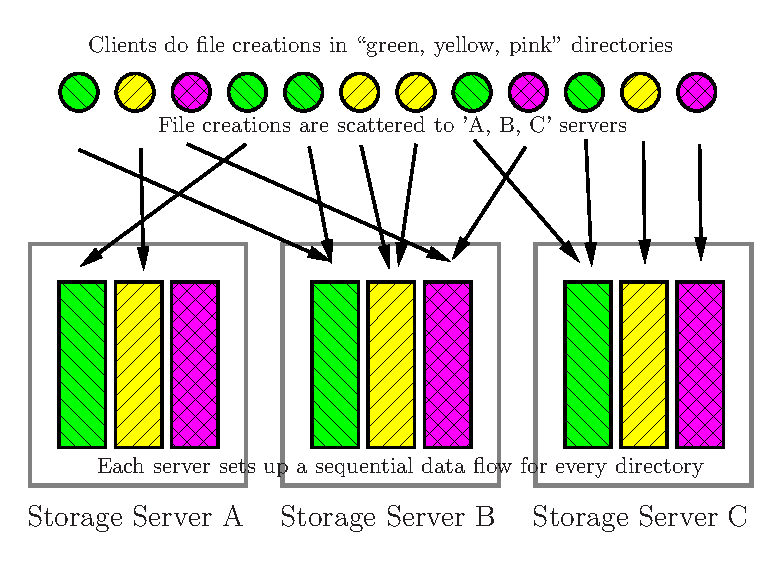
\includegraphics[width=.5\textwidth]{io_write_flow.eps}\\
  \caption{I/O Write Flow: Scatter and Aggregation}\label{io_write_flow}
\end{figure}

    Each server opens one aggregated file for a directory. Instead of in-place modification, file creations and writes are appended to the file. If there are lots of file creations, the creation flow is directed to the file to exploit sequential I/O bandwidth. Temporal continuous data flows (split by column) are transformed to spatial continuous data streams. Further more, because file creations in one directory are scattered to several servers, actually PFS sets up many sequential I/O flows to exhaust concurrent file creations, shown by Figure \ref{io_write_flow}.

    At the same time, columns are stored in separated storage files by default. Thus, each file has already aggregated data content with similar property. For example, in Figure \ref{storage_engine_model}, storage file of column \emph{Medium} contains all files of medium size. For application requests that need to scan all medium images (e.g. violence detection), it is efficient to do sequential reads on the storage file. As columnar store in database, this exploits the vertical spatial locality in directory table.

\section{Experimental Evaluation}

    Our experimental evaluations focus on the typical small file access pattern, and answer three questions: a) Does it save space by adopting CODIR for \emph{NForm} problems? b) What are the metadata and small file performance tradeoffs for our design and implementation choices? c) What lessons we have learned from PFS?

\subsection{Experimental Setup}

    We deploy PFS on two commodity clusters. For cluster A (50 nodes), the hardware configuration of a blade has one quad-core 1.6GHz Intel Xeon processors, 4GB memory, GigE NIC, and connected by 10GigE switches. For cluster B (80 nodes), each blade has three quad-core 1.6GHz Intel Xeon processors, 23GB memory, GigE NIC and switches. Cluster A has a better network, while cluster B has more large memory machines. All nodes were running Linux 2.6.16-60 kernel (Suse release) and PFS stores file system image on a 7200rpm SATA disk.

\subsection{NForm Promblem}

\begin{figure}[t]
  % Requires \usepackage{graphicx}
  \includegraphics[width=.5\textwidth]{eps/spacesavingx.eps}\\
  \caption{Space consumption of saving 1.5 million data contents in PFS, Ext3, OrangeFS. \textit{\small By adopting CODIR, the metadata space consumption is only 1/20 comparing with PFS without CODIR. Meanwhile, CODIR uses less data and metadata space comparing with Ext3 and OrangeFS, and has the lowest latency for this test.}}
  \label{spacesavingx}
\end{figure}

    To find out whether CODIR can save metadata space for \emph{NForm} problem, we run a micro benchmark to write 1,500,000 data contents (total data size is 7.9GB) on one blade of cluster A. For PFS with CODIR, data contents are saved as \emph{three} columns in 500,000 files; for other configurations (PFS without CODIR, Ext3 with \texttt{dir\_index}\footnote{\texttt{dir\_index} option enables hashed-tree indexing for Ext3, and it speeds up the metadata performace.}, and OrangeFS), data contents are saved in 1,500,000 files. Figure \ref{spacesavingx} plots the space consumption of metadata and data and the average write latency. By adopting CODIR, PFS performs best at saving metadata cost, and has the lowest average write latency. Meanwhile, with small file aggregation, the data content are saved continuously. It is more space saving than block based storages such as Ext3 and OrangeFS.

\begin{figure}[t]
  % Requires \usepackage{graphicx}
  \includegraphics[width=.5\textwidth]{eps/gis.eps}\\
  \caption{HTTP performance of a GIS Tile Server based on OrangeFS and PFS. \textit{\small The served HTTP request rate of PFS with CODIR is twice of OrangeFS. With less metadata, file read is more faster.}}
  \label{gis}
\end{figure}

    Second, we setup a GIS tile server\footnote{Tiles are generated from \emph{OpenStreetMap}'s database, and we use TileStach as the HTTP frontend.} which exports a map tile service via HTTP to evaluate the small file read performance. The tile server keeps one million tile images in OrangeFS and PFS. In OrangeFS, the tiles are saved in 1000 subdirectories with 1000 tiles in each subdir. In PFS with CODIR, the tiles are saved in 200,000 files with 5 tiles (columns) in each file. We run \emph{JMeter} to lookup tiles randomly with 10 threads over Giga Ethernet against OrangeFS and PFS based tile server and get the throughput and latency result in Figure \ref{gis}. PFS with CODIR is two times faster than OrangeFS.

    \textbf{Lesson \#1:} CODIR could not only save metadata space, but also increase small file I/O performance.

\subsection{Structured Storage and Interface}

    We used synthetic benchmarks \texttt{cluster postmark} \cite{cluster_postmark} to create, read, append, and delete files to evaluate the small file I/O performance, \texttt{IOZone} to investigate large file I/O, and \texttt{mdtest} to insert zero-byte files in shared directory to evaluate metadata performance.

\subsubsection{File Aggregation}

    % B(ioscal.eps, small_creates, small_read_append), R(spacesavingY.eps)
\begin{figure*}[t]
  % Requires \usepackage{graphicx}
  \includegraphics[width=\textwidth]{eps/ioscale.eps}\\
  \caption{Small File I/O Scalability in Range [1,1K]. \textit{\small Small file write rates increase linearly with more nodes until the servers are saturated. Double the number of servers almost doubles the aggregated file write bandwidth. However, write bandwidth doesn't increase with more servers because of the limited network message rate.}}\label{ioscale}
\end{figure*}

    Firstly, we want to find out the scalability of small file aggregation. We ran \texttt{cluster postmark} in cluster A to investigate the scalability of small file(in range [1,1k]) I/O. In each run, we fixed the number of servers, and variate the number of clients to change loads. Figure \ref{ioscale}(a) plots the file write rate varying with different number of clients and servers. When there were fewer servers, e.g. the \texttt{\#Server=1} line, system saturated quickly and the file write rate is not linearly increasing. When there are more servers, e.g. the \texttt{\#Server=32} line, file write rate keeps increasing linearly. At the same time, in cluster A, we find out that write bandwidth of small files is linear correlated with number of clients if the servers are not saturated(Figure \ref{ioscale}(b)).

    \textbf{Lesson \#2:} Small file ($<$1KB) I/O is linearly scalable with adding more servers and clients.

\begin{figure}[t]
  % Requires \usepackage{graphicx}
  \includegraphics[width=.5\textwidth]{eps/smallcreates.eps}\\
  \caption{Small File Create Rates and Write Bandwidth. \textit{\small For OrangeFS, clients totally creates 4,700,000 files; while for PFS, clients totally creates 47,000,000 files. With increasing the file size, file create rate decreases. The aggregated write bandwidth of PFS with 512KB file is more than 1GB per second.}}\label{smallcreates}
\end{figure}

    Secondly, we want to know whether file aggregation is efficient for concurrent small file creates. We ran \texttt{cluster postmark} (47 processes) in cluster A with file size from 1KB to 512KB, and compared the file create rates and bandwidth between PFS and OrangeFS. Both PFS and OrangeFS were configured with 32 metadata and data servers. Figure \ref{smallcreates} plots the aggregated create rates and write bandwidth. The file create rate and write bandwidth of PFS is more than 6000\% of OrangeFS. By enlarging the file size, file create rates of both file systems are decreasing, while the write bandwidth are increasing. OrangeFS performs worse when small files are larger than 64KB. While, the aggregated write bandwidth of PFS with 512KB files is more than 1GB/s. This bandwidth promotion benefits from our scatter and aggregation small I/O flows in Figure \ref{io_write_flow}.

    \textbf{Lesson \#3:} Directory based small file aggregation plus appropriate I/O scatter framework can greatly improve concurrent small file creation performance.

\begin{figure}[t]
  % Requires \usepackage{graphicx}
  \includegraphics[width=.5\textwidth]{eps/smallio.read.append.eps}\\
  \caption{Small File Read/Append Bandwidth. \textit{\small File read and append bandwidth of PFS is larger than that of OrangeFS. The random read bandwidth of PFS drops at 8KB because the network MTU is only 5100B. Both read and append bandwidth drops at 16KB because PFS client uses 16KB buffer page. More pages means longer latency to read and write. The RMW issue in file append has little impaction on I/O bandwidth.}}\label{smalliora}
\end{figure}

    Thirdly, we want to know how RMW issue affect the small file I/O performance. We ran \texttt{cluster postmark} (75 processes) in cluster B to randomly read or append files (1:1) with file size from 512B to 2MB on PFS and OrangeFS. Both PFS and OrangeFS were configured with 75 metadata and data servers\footnote{OrangeFS failed to run cluster postmark when files are larger than 32KB. This might be a bug of multi-metadata server implementation.}, and \texttt{-noatime} option. Figure \ref{smalliora}\footnote{The aggregated network bandwidth of cluster B is about 200MB/s, and it is limited by the top-level GigEther switch.} plots the I/O bandwidth of file read and append. Both file read and append bandwidth of PFS almost increase with larger file size, and outperform that of OrangeFS. Although there are RMW issues in file append, the append bandwidth increases steadily to the maximum network bandwidth.

    \textbf{Lesson \#4:} RMW issue in file modifications has little impaction on small file I/O performance.

\begin{figure}[t]
  % Requires \usepackage{graphicx}
  \includegraphics[width=.5\textwidth]{eps/spacesavingy.eps}\\
  \caption{Runtime and Space Consumption of Untar 1 million Gene Sequences. \textit{\small Untar short gene sequences in PFS is fastest and most space efficient with respect to OrangeFS and Ceph. This test runs on one machine.}}
  \label{spacesavingy}
\end{figure}

    Finally, we run a real world application to untar 1,000,000 short gene sequence files (most less than 1KB) on PFS, Ceph, and OrangeFS. Ceph is configured to store one data and metadata replica\footnote{We had tried to tune many different configuration variables, Ceph ran slowly still and finished the test in 3 days.}. Figure \ref{spacesavingy} presents the total space consumption and runtime. Benefit from small file aggregation, PFS is much more space efficient and faster than Ceph and OrangeFS. It is 10 times faster than OrangeFS, and the image size is only 19.7\% of OrangeFS and 7.6\% of Ceph.

\subsubsection{Sorted File and Tabular Query}

\begin{figure}[t]
  % Requires \usepackage{graphicx}
  \includegraphics[width=.5\textwidth]{eps/xattr.eps}\\
  \caption{Tag Set and Search Latency. \textit{\small Using sorted file $+$ tabular query interface, tag set and search are faster than external database(BDB) and brute-force scanning search. Especially, external database approach is slow at importing tags to database. And for queries of lower selectivity, sorted file $+$ tabular query performs much more better.}}\label{xattr}
\end{figure}

    In this test, we set up a set of files (1 million) and gave each file a specific tag. For CODIR model, file tags were saved in sorted file; for traditional directory model, file tags were saved in extended attributes; while for database model, file tags were saved in external BerkeleyDB\footnote{The database is configured without transaction support, and in Concurrent Data Store mode(CDB).}. For user queries, we test the tabular query interface, and compare it with brute-force scanning and external database queries. The first two tests perform through \texttt{xattr} syscall interface. Figure \ref{xattr} plots tag set and search latency for different selectivity. Comparing with external BDB approach, using tightly coupled sorted files decreases both tag set and search latency. Comparing with brute-force scanning, database based searches are sensitive to query selectivity. For queries with lower selectivity, it performs more better, because more files are ignored to stat.

    \textbf{Lesson \#5:} Sorted file with tabular query interface performs better than external database indexing and classic directory scanning.

\subsection{Elastic Metadata Service}

    Firstly, we want to find out whether PFS could scale out. We used \texttt{mdtest} to evaluate metadata performance of PFS, GIGA+, OrangeFS, Ceph, and HBase in cluster A. Our configuration used 8 processes per client to simultaneously create files in a shared directory, and the number of files created is proportional to the number of servers: 12.8 million files on 32 servers. HBase is used to simulate the metadata service of Google's next generation file system\cite{gfs}. PFS use FUSE client to complete the test, and each file \texttt{creat()} results in two RPC calls to server: \texttt{getattr()} to check if a file exists, and \texttt{creat()} to create and return file's attributes.

\begin{figure}[t]
  % Requires \usepackage{graphicx}
  \includegraphics[width=.5\textwidth]{eps/mdscale.eps}\\
  \caption{Metadata Scalability of PFS. \textit{\small PFS delivers a peak throughput of roughly 180,000 file creates per second. The network message rate limits PFS's ability to match the ideal linear scalability. It is fast than GIGA+ because of Two-Stage split strategy and none out-of-core indexing.}}
  \label{mdscale}
\end{figure}

    We reuse the experiment results of GIGA+, Ceph, and HBase performed on different clusters from the original paper\cite{giga,ceph}. That cluster used quad-core 2.83GHz machines with 10GigE NICs and switches(faster than ours). Figure \ref{mdscale} compares the aggregated file create throughput, in file creates per second. PFS scales \emph{linearly} up to the size of 32-servers configuration, and can sustain 180,000 file creates per second. PFS also demonstrated scalable performance for the concurrent lookup workload delivering a throughput of more than 410,000 file lookups per seconds(not shown). It benefits from our Two-Stage slice split strategy and removing out-of-core indexing. Although OrangeFS (experimental version) had also implemented a GIGA+ like distributed directories, we found that it performs worse than GIGA+(the bottom line).

    \textbf{Lesson \#6:} By splitting directory and removing out-of-core index, metadata performance imporves greatly.

\subsubsection{Slice Split}

\begin{figure}[t]
  % Requires \usepackage{graphicx}
  \includegraphics[width=.45\textwidth]{eps/splits.eps}\\
  \caption{Local Only, Random, and Two-Stage Splits. \textit{\small Local only splits couldn't exploit more nodes to improve service rate; Random splits introduces too many remote splits and network latency. Both are not efficient slice split strategy for large scale metadata service. Two-Stage splits performs much more better than them.}}\label{splits}
\end{figure}

    Next, we want to find out the metadata behavior of our Two-Stage slice split strategy(firstly split to remote servers, then split at the local servers). The test runs on cluster B with 75 metadata servers and clients. Clients issued millions of file creation requests. Figure \ref{splits} plots the immediate request rate and numbers of two types of splits in three runs with local only, random, and Two-Stage split strategy. It is obviously that Two-Stage splits are far more better than local only and random splits\footnote{To plot the two stage clearly, we slow the transition from remote splits to local splits in Two-Stage strategy intentionally.}. After entering into local split mode, serviced request rate increases for about \emph{10 times} larger.

    \textbf{Lesson \#7:} By exploiting parallelism(more nodes) and locality(local only splits), a simple Two-Stage splits strategy increases the metadata performance greatly.

\subsubsection{Elastic Speedup}

\begin{figure}[t]
  % Requires \usepackage{graphicx}
  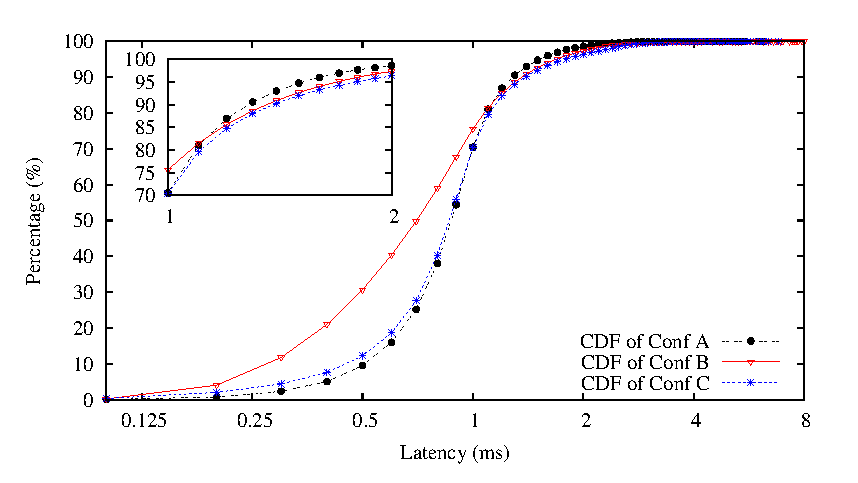
\includegraphics[width=.5\textwidth]{eps/onlineoffline.eps}\\
  \caption{Cumulative Distribution Function of three Runs. \textit{\small Online a server shifts the curve to lower latency(Conf A to B). Offline a server shifts the curve to higher latency(Conf B to C). It means that PFS scales up and down elastically.}}\label{onlineoffline}
\end{figure}

    Finally, we want to find out whether the metadata service of PFS could scale up and down elastically. To understand how server changes impacts on the latency of file operations, we run a test to do file creates, lookups, and removes in three configuration. \texttt{Conf A} ran the test on \emph{one} server without any online/offline operation. In \texttt{Conf B}, we ran the test on one server, and online a new server in the test. In \texttt{Conf C}, we ran the test on two server, and offline an existing server in the test. Figure \ref{onlineoffline} plots the cumulative distribution function of request latency in three configurations. Adding a server made the average request latency smaller, while deleting a server made the latency larger. For \texttt{Conf A,B,C}, half of the requests' latency are under 1ms, and 99\% of them are under 2.2, 2.5, and 2.7ms.

\subsection{Relayed Large File I/O}

\begin{figure*}[t]
  % Requires \usepackage{graphicx}
  \includegraphics[width=\textwidth]{eps/largeio.eps}\\
  \caption{Large File I/O Bandwidth of PFS. \textit{\small With respect to Ext3, PFS FUSE performs bad on both sequential read and write, and introduce 33\% and 15\% overhead. However, comparing with SkyFS in large cluster, PFS performs better.}}\label{largeio}
\end{figure*}

    We want to find out whether our optimizations for small files has affected the large file I/O performance. To understand the tradeoffs of our design choices on large file I/O, we ran \texttt{IOZone} on cluster A to investigate it. In this test, we used Ext3(one node) and SkyFS(30 nodes) as our large file store separately , and all the I/O requests are routed to Ext3 or SkyFS data servers. \texttt{IOZone} is configured with 1MB record size, and the total file size is \emph{three} times larger than memory size. Shown by Figure \ref{largeio}, comparing with Ext3's sequential read, FUSE client of PFS performs bad that the overhead is 33\%. However, comparing with SkyFS, the FUSE client performs better. Because SkyFS also uses FUSE client, we consider that this strange behavior might be some characters of FUSE.

    \textbf{Lesson \#8:} Even considering the FUSE overhead, large file I/O in PFS has not gone bad in large cluster.

\section{Conclusion and Future Work}

    In this paper we address the emerging requirement for large scale small file access. We focus on two common problems: \emph{N-Form} and \emph{1-N Mapping} in distributed file systems, and evolve the directory model, interface and storage structures for small files. We propose to use the tabular directory model and interface. In this way, file system can not only save lots of spaces, but also increase the efficiency of metadata service. On the other hand, we propose to use directory based small file scatter and aggregation. Thus, file system can greatly improve small file I/O performance. Our evaluation shows that by using CODIR model, interface, and storage structures, file system achieves best-in-class performance on a commodity cluster. Especially, metadata and small file performance scale linearly with more nodes.

    PFS is open source at \texttt{github.com} for researchers who want to test, tune or integrate it. In the future, we want to enhance and extend the POSIX interface for small files.

%\section{Acknowledgments}
%
%    \emph{(This Section Intentionally Left Blank for reviewing.)}

% This is where the endnotes (see the ``footnote'' above)
% are filled in.  Use this only if you have endnotes.
% \ifhasendnotes\makeendnotes\fi

\begin{thebibliography}{99}

\bibitem{facebook-haystack} Beaver, Doug and Kumar, Sanjeev and Li, Harry C. and Sobel, Jason and Vajgel, Peter, \emph{inding a needle in Haystack: facebook's photo storage}. Proceedings of the 9th USENIX conference on Operating systems design and implementation (OSDI 2010).

\bibitem{taobao-tfs} Wensong Zhang, \emph{Taobao File System}, \url{http://rdc.taobao.com/blog/cs/?p=128}, (2010).

\bibitem{trf} Rongfeng Tang, Private Communication, (2011).

\bibitem{bigtable} Chang, Fay and Dean, Jeffrey and Ghemawat, Sanjay and Hsieh, Wilson C. and Wallach, Deborah A. and Burrows, Mike, et. al., \emph{Bigtable: a distributed storage system for structured data}, Proceedings of the 7th USENIX Symposium on Operating Systems Design and Implementation, (OSDI 2006)

\bibitem{cstore} Stonebraker, Mike and Abadi, Daniel J. and Batkin, Adam and Chen, Xuedong, et. al., \emph{C-store: a column-oriented DBMS}, Proceedings of the 31st international conference on Very large data bases, (VLDB 2005)

\bibitem{cassandra} Lakshman, Avinash and Malik, Prashant, \emph{Cassandra: a decentralized structured storage system}, SIGOPS Oper. Syst. Rev. vol 44, 35 - 40, (2010)

\bibitem{hbase} HBase, \url{http://hbase.apache.org}, (2010)
\bibitem{ycsb} Cooper, Brian F. and Silberstein, Adam and Tam, Erwin and Ramakrishnan, Raghu and Sears, Russell, \emph{Benchmarking cloud serving systems with YCSB}, Proceedings of the 1st ACM symposium on Cloud computing, (SoCC '10)

\bibitem{lfs} Rosenblum, Mendel and Ousterhout, John K., \emph{The design and implementation of a log-structured file system}, ACM Transactions on Computer Systems, February, (1992)

\bibitem{zfs} \emph{ZFS: the last word in file systems}, Sun Microsystems. September 14, (2004).
\bibitem{wafl} \emph{Network Appliance: File System Design for an NFS File Server Appliance}, NetApp Inc. (1995).
\bibitem{gossip} Andr�� Allavena, Alan Demers and John Hopcroft, \emph{Correctness of a Gossip-based Membership Protocol}, Proc. 24th ACM Symposium on Principles of Distributed Computing (PODC 2005).

\bibitem{ch} Karger, D.; Lehman, E.; Leighton, T.; Panigrahy, R.; Levine, M.; Lewin, D., \emph{Consistent Hashing and Random Trees: Distributed Caching Protocols for Relieving Hot Spots on the World Wide Web}, Proceedings of the 29th Annual ACM Symposium on Theory of Computing, (1997)

\bibitem{reiserfs} Hans Reiser. ReiserFS. \url{www.namesys.com}, (2004).

\bibitem{hotcloud} Patil, S., G.A. Gibson, G.R. Ganger, J. Lopez, M. Polte, W. Tantisiriroj, L. Xiao, \emph{In Search of an API for Scalable File Systems: Under the table or above it?}, USENIX Workshop on Hot Topics in Cloud Computing, (HotCloud 2009)

\bibitem{eh} Fagin, Ronald and Nievergelt, Jurg and Pippenger, Nicholas and Strong, H. Raymond, \emph{Extendible hashing---a fast access method for dynamic files}, ACM Transaction Database System. (1979)

\bibitem{cffs} Ganger, Gregory R. and Kaashoek, M. Frans, \emph{Embedded inodes and explicit grouping: exploiting disk bandwidth for small files}, Proceedings of the annual conference on USENIX Annual Technical Conference, (USENIX ATC 1997)

\bibitem{ceph} Weil, Sage A. and Brandt, Scott A. and Miller, Ethan L. and Long, Darrell D. E. and Maltzahn, Carlos, \emph{Ceph: a scalable, high-performance distributed file system}, Proceedings of the 7th symposium on Operating systems design and implementation, (OSDI 2006)

\bibitem{hfs} Zhang, Zhihui and Ghose, Kanad, \emph{hFS: a hybrid file system prototype for improving small file and metadata performance}, Proceedings of the 2nd ACM SIGOPS/EuroSys European Conference on Computer Systems 2007, (EuroSys 2007)

\bibitem{giga} Swapnil Patil, Garth Gibson, \emph{Scale and concurrency of GIGA+: file system directories with millions of files}, Proceedings of the 9th USENIX conference on File and stroage technologies 2011, (FAST 2011)

\bibitem{skyfs} Xing, Jing and Xiong, Jin and Sun, Ninghui and Ma, Jie, \emph{Adaptive and scalable metadata management to support a trillion files}, Proceedings of the Conference on High Performance Computing Networking, Storage and Analysis, (SC 2009)

\bibitem{nisar} Nisar, Arifa and Liao, Wei-keng and Choudhary, Alok, \emph{Scaling parallel I/O performance through I/O delegate and caching system}, Proceedings of the 2008 ACM/IEEE conference on Supercomputing, (SC 2008)

\bibitem{fuse} FUSE, Filesystem in Userspace, \url{http://fuse.sf.net}/.

\bibitem{cluster_postmark} Lachaize, Renaud and Flouris, Michail, \emph{Parallel Postmark Benchmark: cluster postmark}, \url{http://michail.flouris.net/2008/06/parallel-postmark-benchmark/}.

\bibitem{gfs} McKusick, Marshall Kirk and Quinlan, Sean, \emph{GFS: Evolution on Fast-forward}, ACM Queue, vol 7, 10-20, (2009)

\bibitem{chord} Stoica, Ion and Morris, Robert and Karger, David and Kaashoek, M. Frans and Balakrishnan, Hari, \emph{Chord: A scalable peer-to-peer lookup service for internet applications}, Proceedings of the 2001 conference on Applications, technologies, architectures, and protocols for computer communications, (SIGCOMM 2001)

\bibitem{spyglass} Andrew Leung, Minglong Shao, Timothy Bisson, Shankar Pasupathy, Ethan L. Miller, \emph{Spyglass: Fast, Scalable Metadata Search for Large-Scale Storage Systems}, Proceedings of the 7th USENIX Conference on File and Storage Technologies, (FAST 2009)

\bibitem{smartstore} Yu Hua, Hong Jiang, Yifeng Zhu, Dan Feng and Lei Tian. \emph{SmartStore: A New Metadata Organization Paradigm with Semantic-Awareness for Next-Generation File Systems}, Proceedings of the International Conference for High Performance Computing, Network, Storage and Analysis, ACM/IEEE Supercomputing Conference, (SC 2009)

\bibitem{lustre} P. Schwan, \emph{Lustre: building a file system for 1000-node clusters}, in Proceedings of the Linux Symposium, (2003).

\bibitem{pvfs} Ligon, III, W.B., and Ross, R. B., \emph{PVFS: Parallel Virtual File System}, Beowulf Cluster Computing with Linux, Thomas Sterling, editor, pages 391-430, MIT Press, November, (2001).

\bibitem{europar08} Michael  Kuhn, Julian  Kunkel, Thomas  Ludwig, \emph{Directory-Based Metadata Optimizations for Small Files in PVFS}, Proceedings of the 14th international Euro-Par conference on Parallel Processing, (EuroPar 2008)

\bibitem{ipdps09} Philip Ross Carns, Sam  Lang, Robert Ross Kunkel, Thomas  Ludwig, \emph{Small File Accesses in Parallel File Systems}, Proceedings of the 2009 IEEE International Symposium on Parallel\&Distributed Processing, (IPDPS 2009)

\bibitem{berkeleydb} Oracle, BerkeleyDB, (2011)

\bibitem{lzo} Markus Oberhumer, LZO Compression, \url{www.oberhumer.com/opensource/lzo}, (2011)

\bibitem{dbfs} Nick Murphy and Mark Tonkelowitz and Mike Vernal, \emph{The Design and Implementation of the Database File System}, (2002)

\end{thebibliography}

\end{document}

% Revision History:
% designed specifically to meet requirements of
%  TCL97 committee.
% originally a template for producing IEEE-format articles using LaTeX.
%   written by Matthew Ward, CS Department, Worcester Polytechnic Institute.
% adapted by David Beazley for his excellent SWIG paper in Proceedings,
%   Tcl 96
% turned into a smartass generic template by De Clarke, with thanks to
%   both the above pioneers
% use at your own risk.  Complaints to /dev/null.
% make it two column with no page numbering, default is 10 point

% Munged by Fred Douglis <douglis@research.att.com> 10/97 to separate
% the .sty file from the LaTeX source template, so that people can
% more easily include the .sty file into an existing document.  Also
% changed to more closely follow the style guidelines as represented
% by the Word sample file.
% This version uses the latex2e styles, not the very ancient 2.09 stuff.
%

% Revised July--October 2002 by Bart Massey, Chuck Cranor, Erez
% Zadok and the FREENIX Track folks to ``be easier to use and work
% better''. Hah.  Major changes include transformation into a
% latex2e class file, better support for drafts, and some
% layout improvements.
%%%%%%%%%%%%%%%%%%%%%%%%%%%%%%%%%%%%%%%%%%%%%%%%%%%%%%%%%%%%%%%%%%%%%%%%%%%%%%
% for Ispell:
% LocalWords:  workingdraft BCM ednote SubSections xfig SubSection joe
